
%----------------------------------------------------------------------------------------
%	PACKAGES AND OTHER DOCUMENT CONFIGURATIONS
%----------------------------------------------------------------------------------------
\pdfoutput=1
\documentclass[fleqn,10pt]{SelfArx} % Document font size and equations flushed left

\usepackage[english]{babel} % Specify a different language here - english by default

\usepackage[super,biblabel]{cite} % Superscript citations

\usepackage{setspace} % for block quoting

\usepackage{etoolbox}

\usepackage{graphicx}

\usepackage{algpseudocode}

\AtBeginEnvironment{quote}{\singlespace\vspace{-\topsep}\small}
\AtEndEnvironment{quote}{\vspace{-\topsep}\endsinglespace}

%----------------------------------------------------------------------------------------
%	COLUMNS
%----------------------------------------------------------------------------------------

\setlength{\columnsep}{0.55cm} % Distance between the two columns of text
\setlength{\fboxrule}{0.75pt} % Width of the border around the abstract

%----------------------------------------------------------------------------------------
%	COLORS
%----------------------------------------------------------------------------------------

\definecolor{color1}{RGB}{0,0,90} % Color of the article title and sections
\definecolor{color2}{RGB}{0,20,20} % Color of the boxes behind the abstract and headings

%----------------------------------------------------------------------------------------
%	HYPERLINKS
%----------------------------------------------------------------------------------------

\usepackage{hyperref} % Required for hyperlinks
\hypersetup{hidelinks,colorlinks,breaklinks=true,urlcolor=color2,citecolor=color1,linkcolor=color1,bookmarksopen=false,pdftitle={Title},pdfauthor={Author}}

%----------------------------------------------------------------------------------------
%	ARTICLE INFORMATION
%----------------------------------------------------------------------------------------

% \JournalInfo{..., 2020} % Journal information
% \Archive{arXiv pre-print} % Additional notes (e.g. copyright, DOI, review/research article)

\PaperTitle{JAMPI: efficient matrix multiplication in Spark using Barrier Mode} % Article title

\Authors{Tamas Foldi\textsuperscript{1}*, Chris von Csefalvay\textsuperscript{1}} % Authors
\affiliation{\textsuperscript{1}\textit{Starschema Inc., Arlington, VA.}} % Author affiliation
\affiliation{*\textbf{Corresponding author}: tfoldi@starschema.net} % Corresponding author

% \Keywords{Spark --- Matrix multiplication --- Algorithmic methods} % Keywords - if you don't want any simply remove all the text between the curly brackets
% \newcommand{\keywordname}{Keywords} % Defines the keywords heading name

%----------------------------------------------------------------------------------------
%	ABSTRACT
%----------------------------------------------------------------------------------------

\Abstract{The new barrier mode in Apache Spark allows embedding distributed deep learning training as a Spark stage to simplify the distributed training workflow. In Spark, a task in a stage doesn’t depend on any other tasks in the same stage, and hence it can be scheduled independently. However, several algorithms require more sophisticated inter-task communications, similar to the MPI paradigm. By combining distributed message passing  (using nio/netty), JVM's new \texttt{Vector<>} API and Spark's barrier mode, we can add non-map/reduce based algorithms, such as Cannon's distributed matrix multiplication, improving the performance of the existing MLlib implementation. This paper discloses an efficient distributed matrix multiplication algorithm within a barrier task, which results in an XXX\% performance increase on a 10,000x10,000 square matrix. Applications of efficient matrix multiplication include significantly accelerating the training and implementation of deep convolutional neural network based workloads.}

%----------------------------------------------------------------------------------------

\begin{document}
%\flushbottom % Makes all text pages the same height
\maketitle % Print the title and abstract box
%\tableofcontents % Print the contents section
% \thispagestyle{empty} % Removes page numbering from the first page

%----------------------------------------------------------------------------------------
%	ARTICLE CONTENTS
%----------------------------------------------------------------------------------------

\section{Introduction} % (fold)
\label{sec:introduction}

The recent decade has seen the emergence of two immensely powerful processes in tandem: the rise of big data handling solutions like Apache Spark on one hand and the apotheosis of deep learning as the tool of choice for demanding computational solutions for machine learning problems. Yet at its essence, big data and deep learning remain not only separate communities but also significantly separate domains of software. Despite deep learning over big data becoming a crucial tool in a range of applications, including in computer vision,\cite{guo2016deep,voulodimos2018deep}  bioinformatics,\cite{spencer2014deep,alipanahi2015predicting,zhang2016deep,wei2018prediction} natural language processing (NLP),\cite{deselaers2009deep,socher2012deep,young2018recent,otter2020survey} clinical medicine,\cite{bar2015chest,havaei2016deep,liu2017detecting,stead2018clinical,campanella2019clinical,lehman2019mammographic} anomaly detection in cybersecurity and fraud detection,\cite{du2017deeplog,shone2018deep,chalapathy2019deep} and collaborative intelligence/recommender systems,\cite{wang2015collaborative,deng2016deep,karatzoglou2017deep,batmaz2019review} its full potential remains to be harnessed. The primary impediment in this respect is largely a divergence of attitudes and concerns, leading to two divergent paradigms of development:

\begin{itemize}
	\item \emph{The big data paradigm}, primarily designed around RDDs and the the DataFrame-based API. This outlook has dominated the development of Apache Spark.
	\item \emph{The DL/ML paradigm}, which is primarily focused on efficient linear algebra operations to facilitate machine learning approaches, especially matrix algebra for deep neural networks.
\end{itemize}

The future of deep learning over big data depends greatly on facilitating the convergence of these two worlds into a single, unified paradigm: the use of well-designed big data management tools, such as Apache Spark, to interoperate with the demands of deep learning. The road towards this convergence depends on the development of efficient matrix primitives that facilitate rapid calculations over distributed networks and large data sets.

\begin{figure}
	\centering
	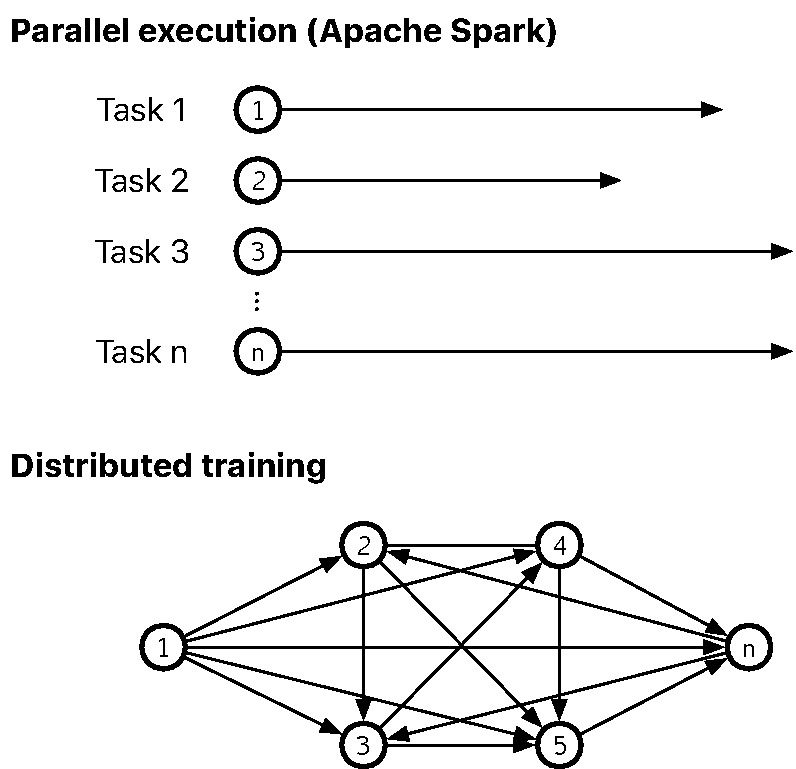
\includegraphics[width=0.9\linewidth]{figures/fig1.pdf}
	\vspace{14pt}
	\caption{Comparative execution models: Apache Spark versus distributed training for neural networks.}
	\label{fig:execution-models}
\end{figure}

The current execution model of Apache Spark is principally focused on independent, embarrassingly parallel tasks that are run and scaled, but the needs of deep learning are primarily focused on distributed training: the performance of completely communicating and coordinating tasks, optimised for interconnectivity rather than independent parallel running, while also maintaining scalability and efficiency. With the recent introduction of the barrier execution mode in Apache Spark, it has finally become possible to construct a computational approach that allows for such networked execution to take place, facilitating distributed training of deep neural networks (see Figure~\ref{fig:execution-models}).

JAMPI (Java Assisted Matrix Product with Inter-task communication), the framework described in this paper, is an efficient and rapid solution to an aspect of efficienty matrix primitives, namely matrix multiplication. By integrating JVM's new \texttt{Vector<>} API, \texttt{nio/netty} for distributed message passing and Spark's barrier mode, a pure Scala implementation of Cannon's 2.5D matrix multiplication algorithm can be devised that is significantly more efficient than \texttt{MLlib}'s \texttt{BlockMatrix.multiply} function. JAMPI thus avoids reliance on low level code on one hand, being a pure Scala implementation. On the other hand, it provides a pre-written framework that integrates with Spark as a native task rather than an external MPI procedure call, and handles inter-task communication directly, yielding performance benefits that would otherwise be associated with a low-level MPI implemented resource negotiation framework.

\subsection{Cannon's algorithm} % (fold)
\label{sub:cannon_s_algorithm}

Matrix multiplication plays a significant role in a range of practical applications, including (but not limited to) scientific computing, non-linear modelling, agent-based models and the training of deep convolutional neural networks (deep learning). The proliferation of deep learning as the cognitive technology of choice for problems with large source data sets and high-dimensional or high-order multivariate data means that efficiency gains in the underlying linear algebra primitives has the potential to enable significant performance benefits in a wide range of use cases. In particular, constructing primitives that leverage computational capacity through rapid parallel computation and efficient interchange lends itself as an avenue towards these performance gains. While packages comprising efficient matrix primitives already exist,\cite{chetlur2014cudnn} these often operate at a low level and do not integrate well with existing and proven solutions to manage large computational loads.


The matrix multiplication operation $\star$ for an $p \times q$ matrix $\mathbf{A}$ and an $q \times r$ matrix $B$ is defined so that for the resultant matrix $\mathbf{C} = \mathbf{A} \star \mathbf{B}$, each element $c_{i, j}$ is the dot product of the $i$-th row of $\mathbf{A}$ and the $j$-th row of $\mathbf{B}$, i.e.

$$ c_{i, j} = \sum_{k = 1}^n a_{i, k} b_{k, j} $$

The multiplication of square matrices constituites a special case. For a square matrix of order $n$, i.e. an $n \times n$ matrix, a special case obtains, which can be resolved efficiently using Cannon's algorithm.\cite{cannon1969cellular} 

For a square matrix of order $n$, i.e. $n \times n$, Cannon's algorithm uses a toroidally connected mesh $\mathbf{P}^{n \times n}$ of $n^2$ processes. Rendered in pseudocode, the algorithm can be expressed as follows for $p$ processors:

\begin{algorithmic}
	\ForAll{i = 0 : $\sqrt{p}$ - 1}
		\State CShift left A[i; :] by i 
	\EndFor
	
	\ForAll{j = 0 : $\sqrt{p}$ - 1}
		\State CShift up B[:; j] by j 
	\EndFor
	
	\For{k = 0 : $\sqrt{p}$ - 1}
		\For{i = 0 : $\sqrt{p}$ - 1, j = 0 : $\sqrt{p}$ - 1}
			\State C[i, j] += A[i, j] * B[i, j]
			\State CShift left A[i; :] by 1
			\State CShift up B[:; j] by 1
		\EndFor
	\EndFor
\end{algorithmic}

Cannon's algorithm is designed to be performed on a virtual square grid $\mathbf{P}$ of $p$ processors (i.e. a $\sqrt{p} \times \sqrt{p}$ matrix). The multiplicand and multiplier matrices $\mathbf{A}$ and $\mathbf{B}$ are laid out on $\mathbf{P}$, after which the $i$-th row of $\mathbf{A}$ is circularly shifted by $i$ to the left and the $j$-th column of $\mathbf{B}$ circularly shifted by $j$ elements up. Then, $n$ times, the two entries mapped onto $p_{i, j}$ are multiplied and added onto the running value of $p_{i, j}$, after which each row of $\mathbf{A}$ is shifted left by one element and each column of $\mathbf{B}$ is shifted up by one element.

Standard methods of multiplying dense matrices require $O(n^3)$ floating operations for an $n \times n$ matrix. Cannon's algorithm improves on this by reducing it to $O(\frac{n^3}{p})$. In particular, because of the fact that memory is not dependent on the number of processors, it scales dynamically with the number of processors. This makes it an attractive candidate for implementation as a high-performance distributed matrix multiplication primitive.

% subsection cannon_s_algorithm (end)

\subsection{Spark's barrier mode} % (fold)
\label{sub:spark_s_barrier_mode}

% subsection spark_s_barrier_mode (end)

% section introduction (end)

\section{Methods} % (fold)
\label{sec:methods}

\subsection{Cannon's algorithm on MPI} % (fold)
\label{sub:cannon_s_algorithm_on_mpi}

% subsection cannon_s_algorithm_on_mpi (end)

\subsection{Matrix multiplication as a barrier task} % (fold)
\label{sub:matrix_multiplication_as_a_barrier_task}

% subsection matrix_multiplication_as_a_barrier_task (end)

\subsection{Vector unrolling} % (fold)
\label{sub:vector_unrolling}

% subsection vector_unrolling (end)

\subsection{Inter-node communication} % (fold)
\label{sub:inter_node_communication}

% subsection inter_node_communication (end)

\subsection{Test protocols} % (fold)
\label{sub:test_protocols}

% subsection test_protocols (end)

% section methods (end)

\section{Results} % (fold)
\label{sec:results}

Comparative analysis of runtimes over a range of matrix sizes reveals that JAMPI is significantly superior (Figure~\ref{fig:runtimes})

\begin{figure}
	\centering
	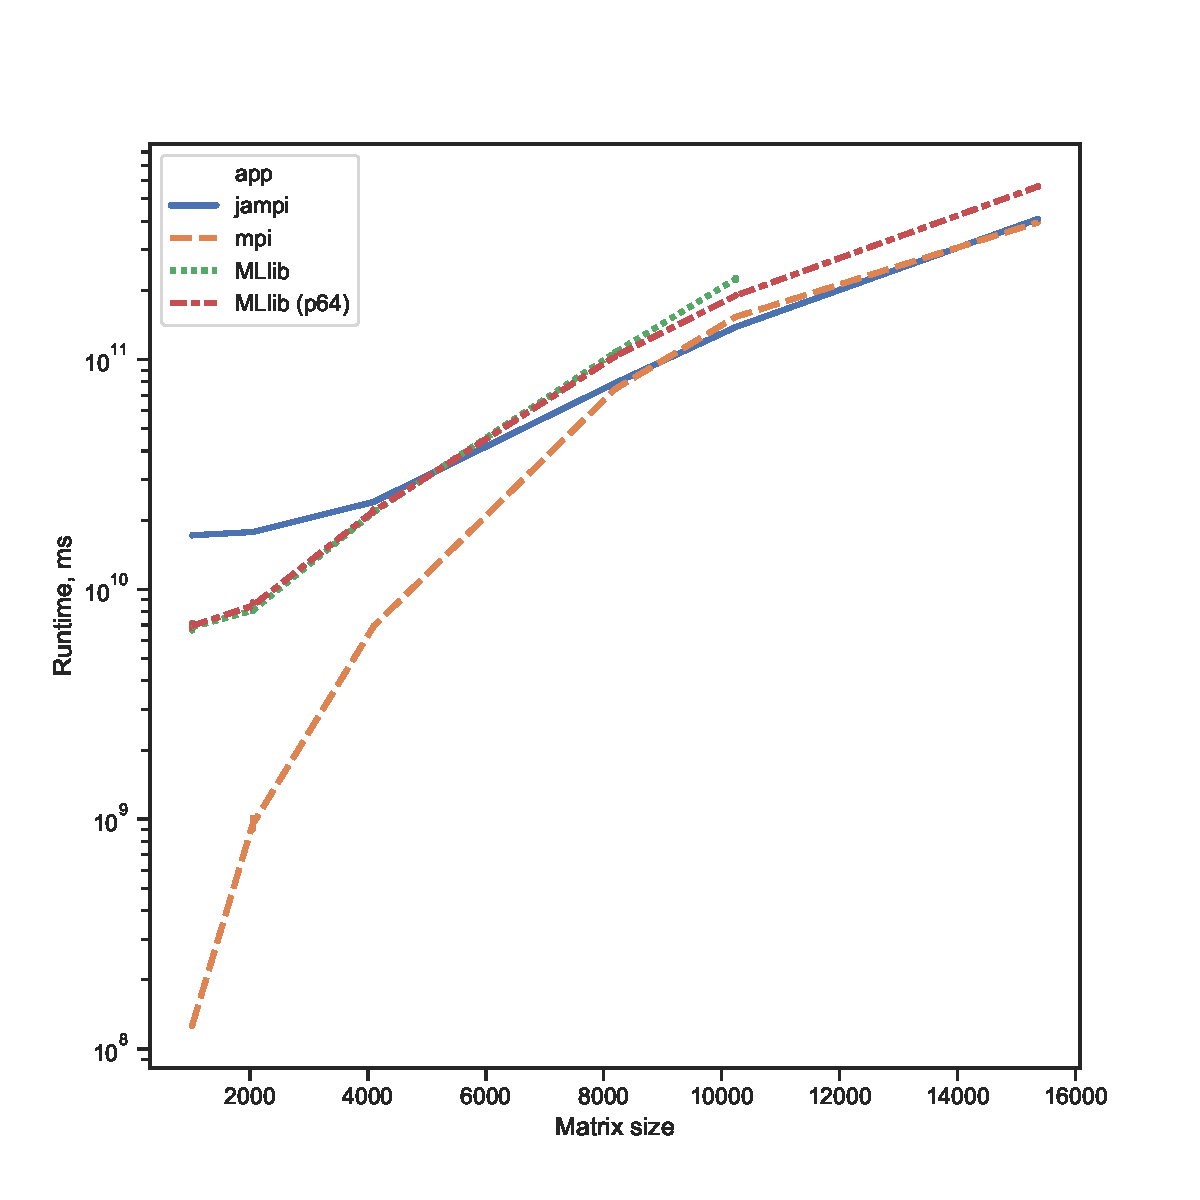
\includegraphics[width=0.9\linewidth]{figures/runtimes.pdf}
	\vspace{14pt}
	\caption{Comparative execution times between JAMPI, MPI, MLlib and MLlib (p64) over $n \times n$ matrices of different sizes.}
	\label{fig:runtimes}
\end{figure}


% section results (end)

\section{Conclusion} % (fold)
\label{sec:conclusion}

% section conclusion (end)

%------------------------------------------------
\phantomsection
\section*{Acknowledgments} % The \section*{} command stops section numbering

% \addcontentsline{toc}{section}{Acknowledgments} % Adds this section to the table of contents

The authors wish to thank Anjan Banerjee for the discussions that inspired this paper. All errors and ommissions are the authors' own.

\phantomsection
\section*{Competing interests} % The \section*{} command stops section numbering

% \addcontentsline{toc}{section}{Acknowledgments} % Adds this section to the table of contents

The authors have declared no competing interest.

\phantomsection
\section*{Funding statement} % The \section*{} command stops section numbering

% \addcontentsline{toc}{section}{Acknowledgments} % Adds this section to the table of contents

The research summarised in this paper was funded by Starschema Inc.


%----------------------------------------------------------------------------------------
%	REFERENCE LIST
%----------------------------------------------------------------------------------------
\phantomsection

\bibliographystyle{unsrt}
\bibliography{bibliography}

%----------------------------------------------------------------------------------------

\end{document}